\subsection{Используемые методы}
\subsubsection{Коррекция фоновой температуры}
\par
Для использования данных фоновой температуры необходимо учитывать два обстоятельства. Во-первых, по сравнению со временем цикла термоанемометра 12 сек температурный датчик имеет довольно значительную тепловую инерцию, равную 1 сек. (более того, мы используем только 2 сек. из 12  в предлагаемом методе анализа данных, как будет видно далее). Во-вторых, датчики термоанемометрии и измерения фоновой температуры находятся в разных приборах каротажной сборки, что приводит к возникновению естественного сдвига во временных рядах при движении этой сборки в потоке флюидов.
\par
Поэтому необходима коррекция данных фоновой температуры как по учету тепловой инерции, так и по проведению увязки по времени данных термоанемометрии и фоновой температуры.
\par
Тепловая инерция измерения температуры определяется \cite{gost} величиной показателя тепловой инерции – времени, необходимого для того, чтобы при внесении датчика в среду с постоянной температурой разность температур среды и датчика составила $e^{-1}\approx0.37$  того значения, которое будет после наступления теплового равновесия. Таким образом, за время измерения с шагом  $\Delta t=1$ сек датчик фоновой температуры $T_{bg}$ с показателем тепловой инерции 1 сек в каждой выбранной точке успевает достичь значения $\alpha(\Delta t)=0.63$ от реальной разницы между текущей и предыдущей точкой.
\par
Поскольку в исследуемом наборе данных фоновая температура записана с неравномерным шагом $\Delta t\in[\Delta t_{min},\Delta t_{max}]$, необходимо вначале построить передаточную функцию $\alpha(\Delta t)$.
Характерный вид кривой разгона термометра показан на рис.\ref{fig:thermal_inertia_curve}(а) \cite{thermal_inertia_patent}. Эту кривую приближенно можно представить как 

\begin{equation}
    T(t) = T_0 \left(1-e^{-\frac{t}{\varepsilon}}\right),
\end{equation}

где $\varepsilon$ - коэффициент тепловой инерции \cite{thermal_inertia_paper}, рис.\ref{fig:thermal_inertia_curve}(б). Так как для выбранного датчика $\varepsilon=1$с, то для рассматриваемого датчика получаем 

\begin{equation}
    \alpha(\Delta t) = 1 - e ^ {-\Delta t}
\end{equation}

\begin{figure}[H]
\centering
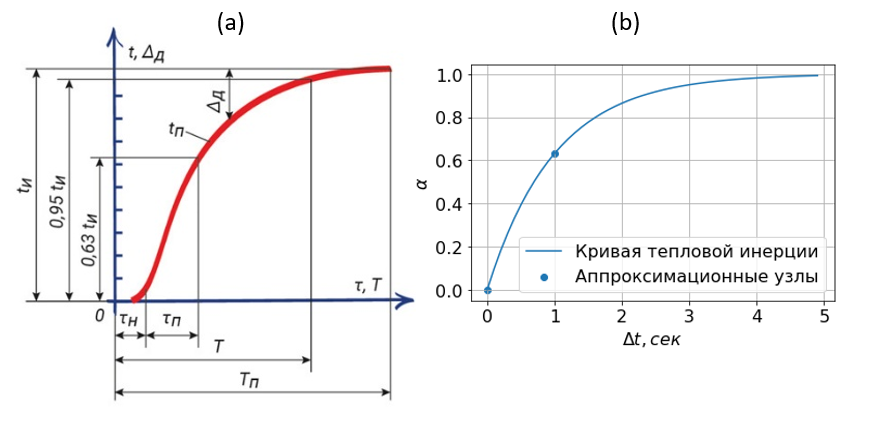
\includegraphics[width=1.0\textwidth]{TA/thermal_inertia_curve.png}
\caption{Характерный (a) и аналитический (b) виды кривой разгона термометра (передаточной функции). Для используемого датчика $\tau_H+\tau_\Pi=1$.}
\label{fig:thermal_inertia_curve}
\end{figure}

\par
Для вычисления «истинной» фоновой температуры $T_{bg}(t^i)$ обозначаем данные показаний датчика фоновой температуры через $T_d(t^i)$ и составляем следующее уравнение:
\begin{equation}
    T_{bg}(t^{i+1})-T_d(t^{i+1})=    \left(1-\alpha\right)\left(T_{bg}(t^{i+1})-T_{bg}(t^i)\right)
\end{equation}
Из него получаем формулу вычисления фоновой температуры:
\begin{equation}
    T_{bg}(t^{i+1})=T_{bg}(t^i)+\frac{T_d(t^{i+1})-T_x{bg}(t^i)}{\alpha}
\end{equation}

Результат работы алгоритма на некотором участке временного ряд для 50 точек показан на рис.\ref{fig:thermal_inertia_result}.
\begin{figure}[H]
\centering
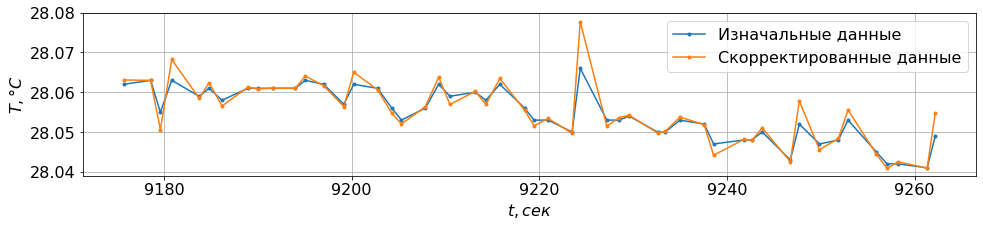
\includegraphics[width=1.0\textwidth]{TA/thermal_inertia_result.png}
\caption{Результат работы алгоритма коррекции тепловой инерции на 50 точках.}
\label{fig:thermal_inertia_result}
\end{figure}
\par
Для коррекции естественного сдвига во временных рядах данных термоанемометрии и фоновой температуры при движении сборки приборов в потоке флюидов мы вводим расстояние $L$ по стволу скважины между датчиками и относительную скорость $V$ приборов и потока. Тогда, очевидно, искомый сдвиг по времени $\delta t$ оценивается как
\begin{equation}
    \delta t = \frac{L}{V},
\end{equation}

а вычисление значений $T_{bg}(t^i-\delta t)$ проводится линейной интерполяцией.

\par
Полученные значения фоновой температуры используются для решения задачи разделения флюидов совместно с данными термоанемометра, рассматриваемой в следующем параграфе.

\subsubsection{Анализ данных распределенного термоанемометра}
\par
Рассматривается задача определения фазы флюида для каждого цикла. Экспериментальные исследования показывают, что форма циклов зависит от скорости флюида и его физических характеристик, см. рис.\ref{fig:cycle_examples_dem}.

\begin{figure}[H]
\centering
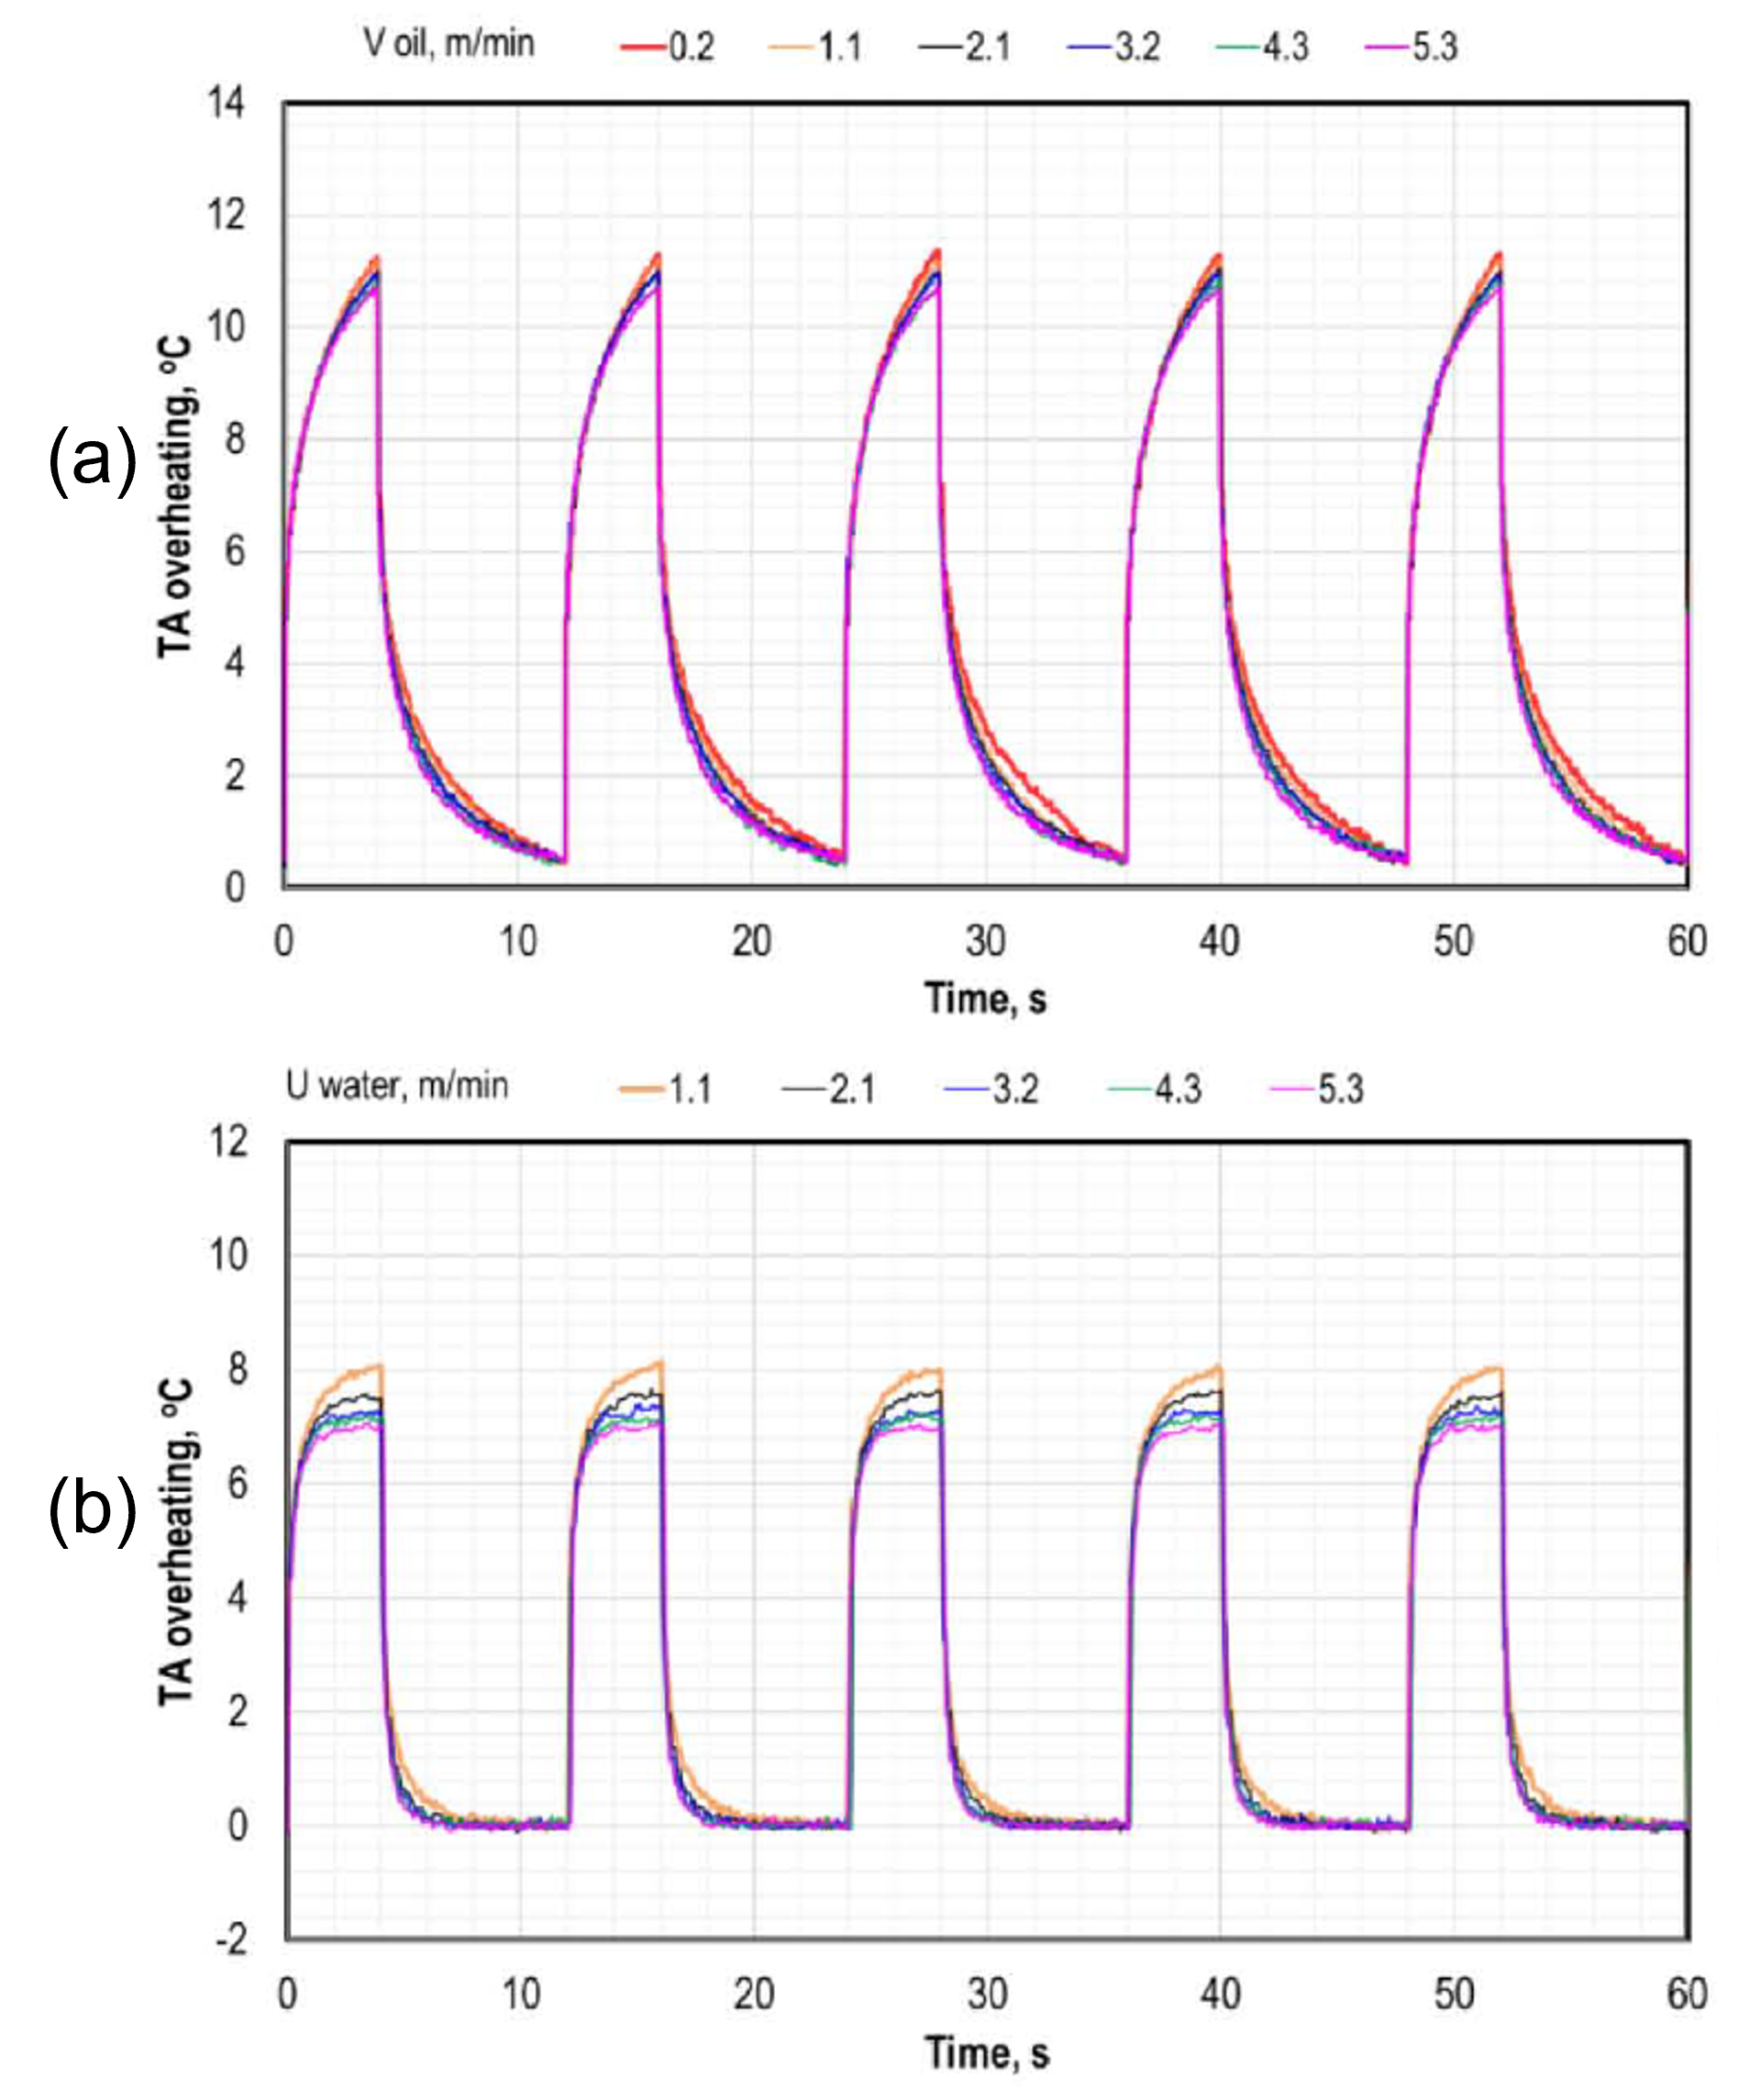
\includegraphics[width=0.6\textwidth]{TA/cycle_examples_dem.png}
\caption{Характерные циклы нагревания-охлаждения для нефти (a) и газа (b) при различных скоростях потока на протяжении пяти последовательных циклов. Лабораторные данные, результаты статьи \cite{horizonal_1}.}
\label{fig:cycle_examples_dem}
\end{figure}

\par
Изменения скорости и характеристик флюидов в определенных пределах могут вызывать изменения численных характеристик кривой графика также в определенных пределах, присущих каждому из трех типов циклов. Назовем такие численные характеристики индикаторами. Например, используются следующие индикаторы:

\begin{enumerate}
    \item[$I_1$] - разность максимальной и минимальной температур цикла
    \item[$I_2$] - производная кривой цикла в конце фазы охлаждения
    \item[$I_3$] - производная кривой цикла в конце фазы нагревания
    \item[$I_4$] - интеграл кривой цикла на протяжении фазы охлаждения
    \item[$I_5$] - интеграл кривой цикла на протяжении фазы нагревания
\end{enumerate}
и другие.
\par
На данный момент процесс интерпретации данных термоанемометрии на основе  и некоторых других (в том числе, лабораторных) измерений включен в алгоритм обработки ПГИ данных \cite{horizonal_1},\cite{horizonal_2}.
\par
Из рис.\ref{fig:cycle_examples_dem} видно, что практически все указанные индикаторы хорошо различают две фазы (нефть, вода) независимо от рассмотренных значений скорости потока. Однако, если скорости и параметры флюида претерпевают значительные изменения, то и интервалы изменений индикаторов могут пересекаться для различных фаз. Можно также отметить и другие проблемы обработки измерений, усугубляющие неоднозначность соответствия какого-либо индикатора определенной фазе, например:
\begin{itemize}
    \item Все датчики термоанемометрии немного отличаются, требуется калибровка
    \item Использование лабораторных данных требует знания характеристик флюидов и корректировки на скважинные условия
    \item Распознавание газовой фазы вызывает затруднение из-за близости значений индикаторов для нефти и газа во многих случаях
    \item За время цикла 12 сек может произойти смена фаз, что приводит к неоднозначности интерпретации индикаторов
\end{itemize}
\par
Цель исследования - уменьшение влияния указанных проблем на результаты распознавания фаз воды, нефти и газа (в идеале – исключения влияния). Важным условием является также и то, что разрабатываемый метод не должен использовать экспертную разметку данных, поскольку она недоступна в необходимом объеме, например, для алгоритмов обучения с учителем.
\par
В результате исследований поведения различных циклов из используемого датасета мы разработали метод обработки измерений, в котором подобраны индикаторы и составлены из них комбинации, т.е. признаки, позволившие использовать методы кластеризации для достаточно четкого распознавания всех трех фаз.

\paragraph{Создание признакового пространства.} 
\par
Для построения алгоритма анализировались скважинные данные примерно 1500 циклов одного из датчиков. Обозначим температуру одного цикла как $T(t_i),\;i=1,...,120$. Для упрощения обозначений мы опускаем индексы номера цикла и номера датчика из датасета и полагаем, что время соответствует абсолютному значению в датасете.  В течение интервала записи данных цикла (12 секунд) датчик может перейти из одной фазы в другую. Чтобы уменьшить вероятность влияния этого события на результат, мы используем только небольшую часть цикла для построения индикаторов, и рассматриваем точки из интервала $i=40,...,59$, т.е. 2 секунды. Это включает в себя последнюю точку фазы нагревания $i=40$ и начало фазы охлаждения. Поскольку замеры искажены случайным шумом, мы аппроксимируем точки фазы охлаждения  параболой для вычисления значений температуры и ее производной в первой точке фазы охлаждения. Обозначим эту параболу через $T^C(t)$. 
\par
После анализа, в том числе и путем перебора, в качестве индикаторов были выбраны
\begin{equation}
    T(t_{40}),\quad T^C(t_{41}),\quad \frac{dT^C}{dt}(t_{41}),\quad T_{bg}(t_{41}),
\end{equation}

где $T_{bg}$ - фоновая температура, вычисляемая согласно алгоритму из предыдущего параграфа.
\par
Чтобы уменьшить влияние скважинных условий и отличий характеристик датчиков, мы проводим обезразмеривание по температуре и формируем два признака из предложенных четырех индикаторов:

\begin{equation}
    F_1 = \frac{\frac{dT^C}{dt}(t_{41})}{T(t_{40})-T^C(t_{41})},\quad F_2 = \frac{T(t_{40})-T_{bg}(t_{41})}{T(t_{40})-T^C(t_{41})}
\end{equation}
\par
Признаки имеют простой физический смысл: $F_1$ с размерностью $\left[\frac{1}{\text{сек}}\right]$ характеризует скорость начала охлаждения, а безразмерный  $F_2$ характеризует масштаб перепада температур после окончания нагрева. Отметим, что в обезразмеривании по времени (т.е., исключении $\left[\frac{1}{\text{сек}}\right]$) нет необходимости, так как шаг по времени 0.1 сек в цикле измерений фиксирован для всех датчиков.
На рис.\ref{fig:sensor_1_raw_data}(а) в координатах $\left(F_1, F2\right)$ построены точки для измерений одного из датчиков.  Отчетливо видны три облака с приведенными условными границами (линии), которые могут соответствовать трем типам флюидов – воде, нефти и газу. Отметим достаточно изотропную форму каждого из облаков. На карте плотности точек, рис.\ref{fig:sensor_1_raw_data}(б), хорошо высвечиваются «водяной» и «нефтяной» кластеры («газовый» кластер практически не высвечивается из-за существенно меньшего количества точек в нем).

\begin{figure}[H]
\centering
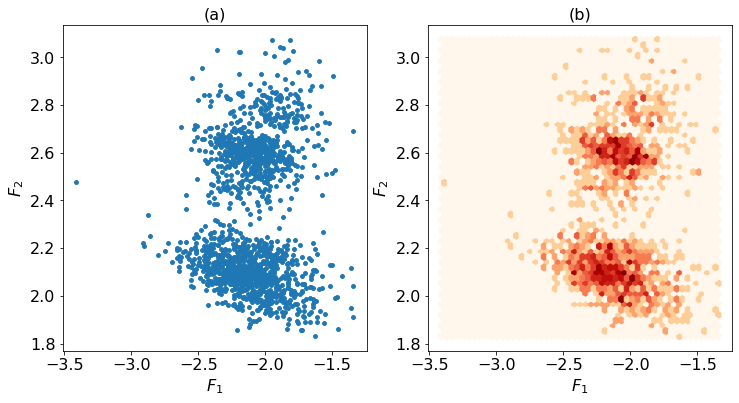
\includegraphics[width=0.8\textwidth]{TA/sensor_1_raw_data.png}
\caption{Скважинные данные термоанемометра для одного из датчиков (около 1500 точек) в координатах предложенных признаков (а) и их раскраска в соответствии с плотностью точек (б)}
\label{fig:sensor_1_raw_data}
\end{figure}

\paragraph{Кластеризация признакового пространства}
Разделение данных в полученном пространстве на три кластера делается с помощью модели смеси гауссовских распределений. Так как верхний кластер, который мы будем обозначать как «газ», содержит существенно меньше точек, и он гораздо ближе к среднему кластеру, который мы будем обозначать как «нефть», то кластеризация проводится в два этапа:
\begin{itemize}
    \item[1.] Модель 1 классификации на 2 гауссовских распределения отделяет нижний кластер («вода») от двух верхних.
    \item[2.] Оставшиеся после удаления нижнего кластера данных разделяются моделью 2 классификации на 2 гауссовских распределения на два кластера – «нефть» и «газ».
\end{itemize}

Процесс создания итоговой разметки продемонстрирован на рис.\ref{fig:sensor_1_clustering_process}. 

\begin{figure}[H]
\centering
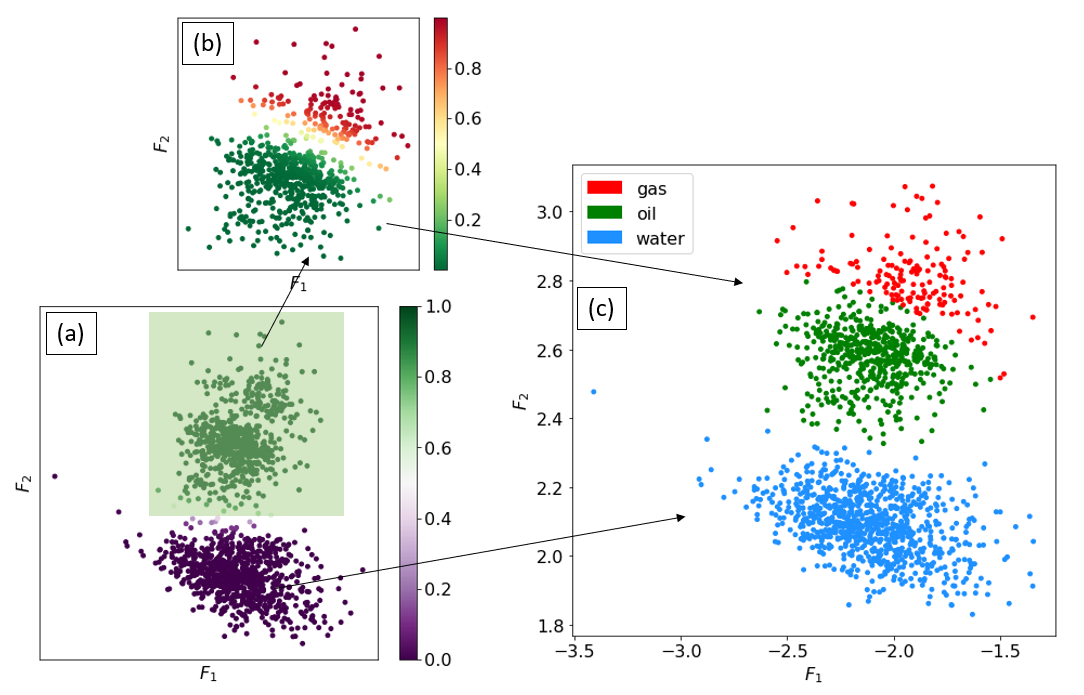
\includegraphics[width=1.0\textwidth]{TA/sensor_1_clustering_process.png}
\caption{Процесс создания итоговой разметки. Сначала (a) нижний водяной кластер отделяется от верхнего; верхний кластер разделяется (b) на нефть и газ. Полученные в результате работы двух GMM-моделей метки объединяются в итоговую (c).}
\label{fig:sensor_1_clustering_process}
\end{figure}

\paragraph{Определение положения и фазового состава точек смены фаз}
\par
Переход между фазами, то есть изменение характеристик цикла, соответствует переходу между кластерами в координатах $\left(F_1, F2\right)$. Пример перехода между фазами продемонстрирован на рис.\ref{fig:sensor_1_phase_change_demo}.  Раскраска точек соответствует полученной ранее дискретной разметке. Справа показаны восемь последовательно измеренных циклов, на основном графике стрелками тех же цветов соединяются точки в координатах $\left(F_1, F2\right)$, соответствующие этим циклам. Прибор двигался от меньшего номера цикла к большему, то есть от голубого цвета к розовому. Видно, что изменения формы циклов нагревания-охлаждения соответствуют перемещениям в выбранном пространстве признаков.

\begin{figure}[H]
\centering
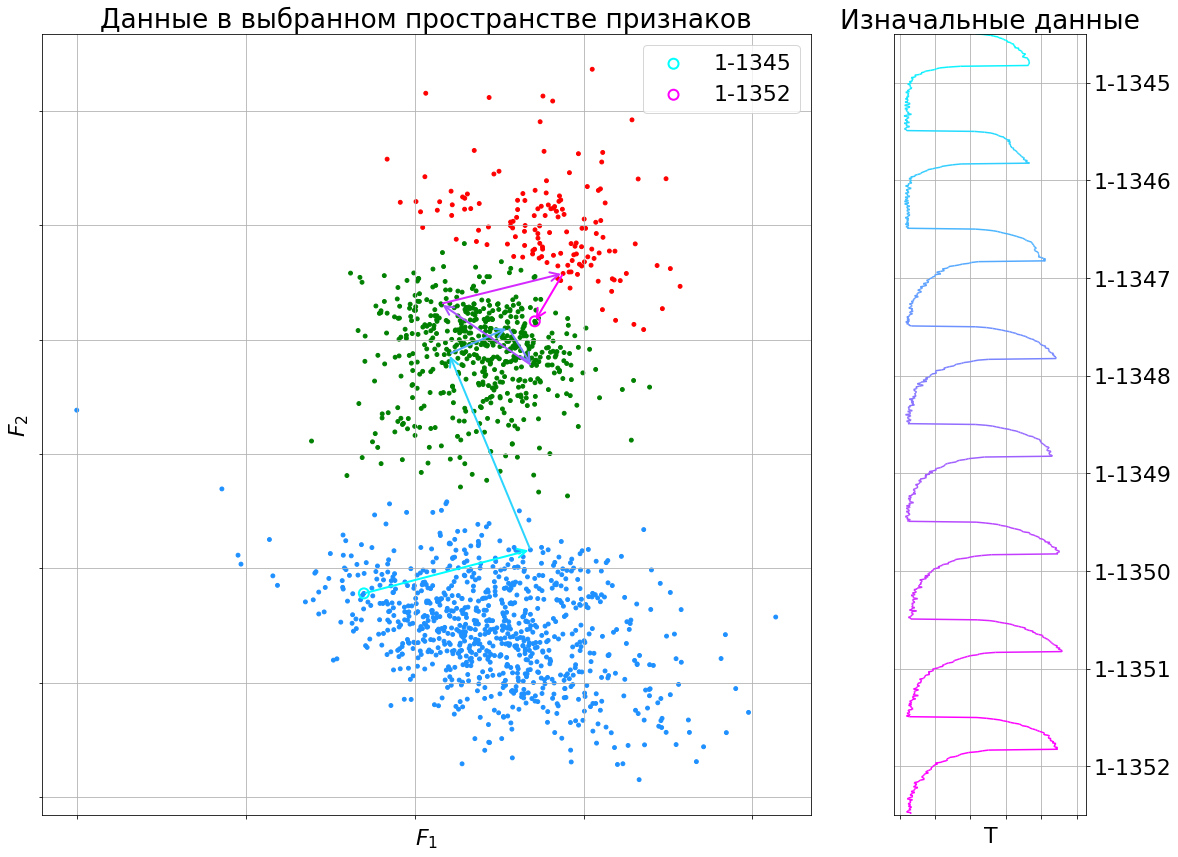
\includegraphics[width=1.0\textwidth]{TA/sensor_1_phase_change_demo.png}
\caption{Демонстрация того, как точки переходят между фазами. На правой колонке видно, как на протяжении 8 циклов меняется форма цикла - и это отражается движением точек, соответствующих этим циклам в выбранном признаковом пространстве. Движение начинается с голубого цикла, находящегося в водяном кластере, и заканчивается в розовом цикле, находящимся на границе нефтяного и газового кластера.}
\label{fig:sensor_1_phase_change_demo}
\end{figure}

\par
Необходимо автоматически определять точки смены фаз и присваивать им оценку фазового состава флюидов.
Так как разделение на кластеры производится вероятностной моделью, то дискретные метки вода-нефть-газ получаются из вероятностных оценок нахождения выбранной точки датасета в каждой из фаз. Так как разделение делается дважды: сначала отделяется вода, а потом разделяются нефть и газ, то на самом деле «сырой» результат работы модели – это два набора вероятностей.  
\par
Поэтому:
\begin{enumerate}[label=\arabic*.]
    \item Для каждой точки из класса «вода» доступны вероятности $p_{water}^1$ и $p_{oil}^1$ такие, что $p_{water}^1+p_{oil}^1=1$.
    \item Для каждой точки из класса «нефть» доступны вероятности $p_{water}^1$ и $p_{oil}^1$ такие, что $p_{water}^1+p_{oil}^1=1$; а также вероятности $p_{oil}^2$ и $p_{gas}^2$ такие, что $p_{oil}^2+p_{gas}^2=1$.
    \item Для каждой точки из класса «газ» доступны вероятности $p_{oil}^2$ и $p_{gas}^2$ такие, что $p_{oil}^2+p_{gas}^2=1$.
\end{enumerate}

\par
Форма и процесс получения выделяемых кластеров в координатах $\left(F_1, F2\right)$ предполагает только два варианта точек смены фаз: «вода-нефть» и «нефть-газ»; вариант «вода-газ» не выделяется, так как соответствующие кластеры получаются двумя различными смесями распределений.

\par
Предложен и реализован следующий алгоритм выделения точек смены фаз и оценки фазового состава. Для модели 1 (отделение воды от нефти и газа) задаются пороги $thr_{water}^1$ и $thr_{oil}^1$ такие, что $0\leq thr_{water}^1 \leq 1$ и $0\leq thr_{oil}^1 \leq 1$, при этом для существования точек смены фаз необходимо выполнение условия $thr_{water}^1+thr_{oil}^1\geq 1$. Для каждого набора вероятностей $(p_{water}^1,p_{oil}^1)$  в зависимости от значений выбранных порогов создается метка M:
\paragraph{Алгоритм для модели 1}
\begin{enumerate}[label=\arabic*.]
    \item Если $thr_{water}^1 \leq p_{water}^1$, то M = «вода».
    \item Если $1-thr_{oil}^1< p_{water}^1<thr_{water}^1$, то M = «$p_{water}^1$\% вода+$p_{oil}^1$\% нефть».
    \item Если $p_{water}^1\leq 1-thr_{oil}^1$, то ТM=«нефть».
\end{enumerate}
	
\par
Гистограмма распределения значений $p_{oil}^1$ для датчика 1 показана на рис.\ref{fig:histogram_1}. Для примера указаны значения $thr_{water}^1= thr_{oil}^1=0.9$. Видно, что по результату работы описанного выше алгоритма большая часть точек приобретет метку «вода» (синяя зона) или «нефть» (зеленая зона), в то время как небольшое количество точек в голубой зоне будут классифицированы как смесь флюидов.
 
\begin{figure}[H]
\centering
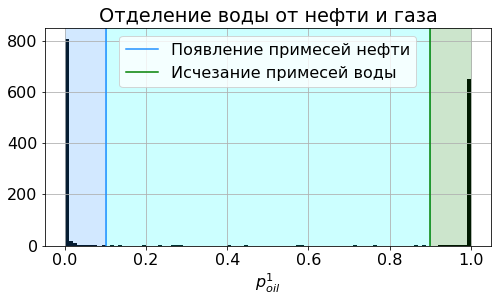
\includegraphics[width=0.8\textwidth]{TA/histogram_1.png}
\caption{Распределение значений вероятностей точек не попасть в водяной кластер. Видно, что разделение сильно бимодальное - про большинство точек мы можем с уверенностью сказать, в какой фазе они находятся; но присутствуют и точки между прямыми линиями - им мы присваиваем оценку фазового состава вода+нефть.}
\label{fig:histogram_1}
\end{figure}
\par
Аналогичная процедура проводится для модели 2 (отделение нефти от газа). Задаются пороги $thr_{oil}^2$ и $thr_{gas}^2$ такие, что $0\leq thr_{oil}^2\leq 1$ и $0\leq thr_{gas}^2\leq 1$, при этом для существования точек смены фаз необходимо выполнение условия $thr_{oil}^2+thr_{gas}^2\geq 1$.
\paragraph{Алгоритм для модели 2}
\begin{enumerate}[label=\arabic*.]
	\item Если $thr_{gas}^2\leq p_{gas}^2$, то M = «газ».
	\item Если $thr_{oil}^2< p_{gas}^2<thr_{gas}^2$, то M = «$p_{oil}^2$\% нефть+$p_{gas}^2$\% газ».
	\item Если $p_{gas}^2\leq 1-thr_{oil}^2$, то M=«нефть».
\end{enumerate}	
\par
Гистограмма распределения значений $p_{gas}^2$ для датчика 1 показана на рис.\ref{fig:histogram_2}. Для примера указаны $thr_{oil}^2=thr_{gas}^2=0.9$. Видно, что по результату работы описанного выше алгоритма большая часть точек приобретет метку «нефть» (зеленая зона) или «газ» (красная зона), в то время как небольшое количество точек в желтой зоне будут классифицированы как смесь флюидов.

\begin{figure}[H]
\centering
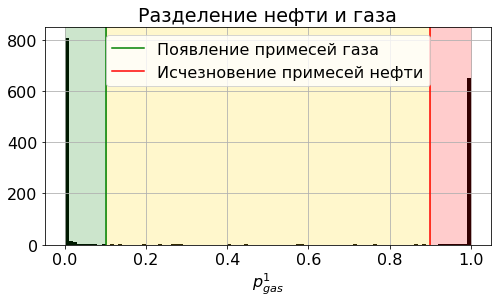
\includegraphics[width=0.8\textwidth]{TA/histogram_2.png}
\caption{Разделение нефти и газа происходит аналогично работе модели 1. Здесь распределение опять бимодальное - у большинства точек с уверенностью определяется фаза. Здесь, как и на предыдущей гистограмме, задаются отсечки между дискретной фазой и смесью флюидов.}
\label{fig:histogram_2}
\end{figure}

\par
Так как каждая точка, классифицированная как нефть, имеет как вероятность $p_{water}^1$ содержать какую-то часть воды, так и вероятность $p_{gas}^2$ содержания газа, то выбор алгоритма для модели 1 или модели 2 (то есть классификация точки как смеси «вода+нефть» либо «нефть+газ») определяется из сравнения этих вероятностей: если $p_{oil}^1>p_{oil}^2$, то используется алгоритма для модели 1, и наоборот.
\par
Полученные точки смены фаз показаны на рис.\ref{fig:sensor_1_final}(a) желтым и голубым цветами; раскраска соответствует гистограммам.
\par
На рис.\ref{fig:sensor_1_final}(b) представлена финальная разметка с оценкой фазового состава в точках смены фаз.

\begin{figure}[H]
\centering
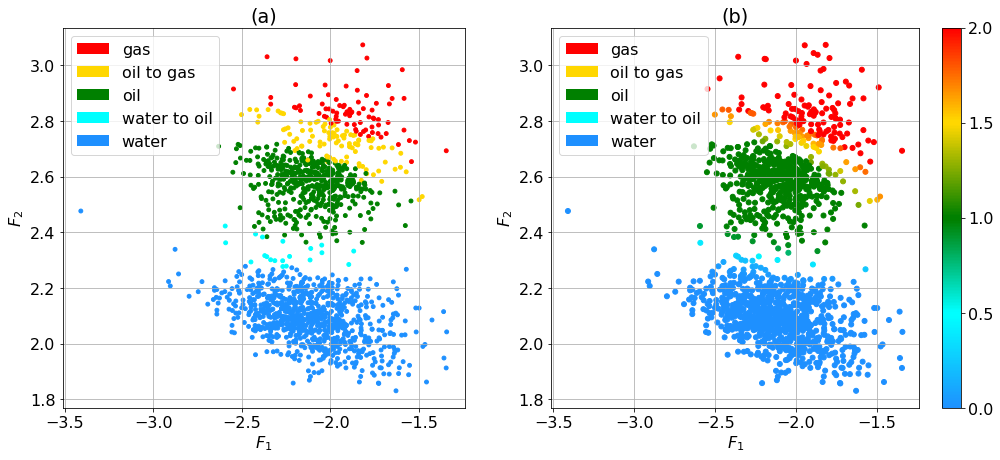
\includegraphics[width=1.0\textwidth]{TA/sensor_1_final.png}
\caption{На (a) - отделение точек смены фаз от точек, содержащих одну фазу, в соответствии с определенными ранее порогами. На (b) - то же разделение, но точкам смены фаз присвоены пропорции фазового состава.}
\label{fig:sensor_1_final}
\end{figure}